% Fresnel paper for ISWC05

% based on LLNCS.DEM the demonstration file of
% the LaTeX macro package from Springer-Verlag
% for Lecture Notes in Computer Science,
% version 2.2 for LaTeX2e
%
\documentclass{llncs}
%
\usepackage{makeidx}  % allows for indexgeneration
\usepackage{graphicx}
%
\begin{document}
%
\newcommand{\rdf}[1]{{\small \texttt{#1}}}

\frontmatter          % for the preliminaries
%
\pagestyle{headings}  % switches on printing of running heads
\mainmatter              % start of the contributions
%
\title{Fresnel - A Browser-Independent Presentation Vocabulary for RDF}
%
\titlerunning{Fresnel - A browser-independent Presentation Vocabulary for RDF}
% abbreviated title (for running head)
%                                     also used for the TOC unless
%                                     \toctitle is used
%
\author{Christian Bizer\inst{1} \and Ryan Lee\inst{2} \and Emmanuel Pietriga\inst{3}}
%
%\authorrunning{Bizer et al.}   % abbreviated author list (for running head)
%
%%%% modified list of authors for the TOC (add the affiliations)
\tocauthor{Chris Bizer (Berlin),
Ryan Lee (MIT),
Emmanuel Pietriga (INRIA)}
%
\institute{Freie Universit\"at Berlin, Germany \\
\email{chris@bizer.de}
\and
W3C/MIT CSAIL, Cambridge, USA\\
\email{ryanlee@w3.org}
\and
INRIA \& Laboratoire de Recherche en Informatique (LRI), Orsay, France\\
\email{emmanuel.pietriga@inria.fr}
}

\maketitle

%--------------------------------------------------------------------
\begin{abstract}
Semantic Web browsers and other tools aimed at displaying RDF data to end users are all concerned with the same problem: presenting content primarily intended for machine consumption in a human-readable way. Their solutions differ but in the end address the same two high-level issues, no matter the underlying representation paradigm: specifying (i) {\em what} information contained in RDF models should be presented (content selection) and (ii) {\em how} this information should be presented (content formatting and styling). However, each tool currently relies on its own {\em ad hoc} mechanisms and vocabulary for specifying RDF presentation knowledge, making it difficult to share and reuse such knowledge across applications. Recognizing the general need for presenting RDF content to users and wanting to promote the exchange of presentation knowledge, we developed Fresnel as a browser-independent extensible vocabulary of core RDF display concepts.
\end{abstract}

%--------------------------------------------------------------------
%--------------------------------------------------------------------
\section{Introduction}

Software agents are the primary consumers of Semantic Web content. RDF is thus designed to facilitate machine interpretability of information and does not define a visual presentation model since human readability is not one of its stated goals. However, RDF applications are not only about the semantic processing of information. Information coming from the Semantic Web, either directly from RDF repositories or as a result of complex processes, often must be presented to users. Displaying RDF data in a user-friendly manner is a problem addressed by various types of applications using different representation paradigms. Tools like IsaViz \cite{isaviz} and Welkin \cite{Welkin} represent RDF models as node-link diagrams, explicitly showing their graph structure. Other tools use nested box layouts (Longwell \cite{simile}) or table-like layouts (Brownsauce \cite{Steer03}, Noadster \cite{Rutledge05}, Swoop \cite{MindSwap05}) for displaying properties of RDF resources with varying levels of details. A third approach combines these paradigms and extends them with specialized user interface widgets designed for specific information items like calendar data, tree structures, or even DNA sequences, providing advanced navigation tools and other interaction capabilities (Haystack \cite{Quan04}, mSpace\cite{mspace2005}).

Such applications are confronted with the same two issues, independently of the underlying representation paradigm and interface capabilities: selecting what content to show and specifying how to format and style this content. Each application takes its own approach and defines its own vocabulary to specify how to present data to users. As with other kinds of knowledge, we believe that being able to share what we consider {\em presentation knowledge} makes sense in the context of the Semantic Web and that being able to exchange and reuse presentation knowledge between browsers and other visualization applications will benefit both programmers and end users. However, the current diversity of approaches and vocabularies for representing this knowledge makes such exchange and reuse difficult at best, if not impossible.

\subsection{Current methods for specifying presentation knowledge}

Early RDF visualization tools rendered RDF models in a predefined, non-custo\-mizable way \cite{Steer03}. Recent tools provide more flexible visualizations that can be customized by writing style sheets, transformations, or templates, following either a declarative or a procedural approach.

Procedural approaches consider the presentation process as a series of transformation steps. One such approach consists of using XSLT to transform RDF graphs encoded as RDF/XML trees in an environment such as Cocoon \cite{cocoon05}. Authoring XSLT templates and XPath expressions to handle arbitrary RDF/XML is complex, if not impossible, considering the many potential serializations of a given RDF graph and the present lack of a commonly accepted RDF canonicalization in XML \cite{Carroll04}. This problem has been partly addressed by Xenon \cite{quan05}, an RDF style sheet ontology that builds on the ideas of XSLT but combines a recursive template mechanism with SPARQL as an RDF-specific selector language. Xenon succeeds in addressing XSLT's RDF canonicalization problem but still has a drawback common to all procedural approaches, that transformation rules are tied to a specific display paradigm and output format preventing the reuse of presentation knowledge across applications.

Declarative approaches are based on formatting and styling rules applied to a generic representation of the content. They can be compared to XHTML+CSS, which has been successful for the classic Web. The Haystack Slide ontology \cite{HaystackUI03}, used to describe how Haystack display widgets are laid out, is one example. Another is IsaViz's Graph Style Sheets \cite{gss03}, which modifies the formatting, styling, and visibility of RDF graph elements represented as node-link diagrams. The main drawback of the declarative approaches developed so far is that they make strong assumptions about, and are thus tied to, the specific display paradigm for which they have been developed and are therefore unlikely to be meaningful across different representation paradigms.

\subsection{Toward the specification of presentation knowledge}

Providing a single global view of all the information contained in an RDF model is often not useful. The amount of data makes it difficult to extract information relevant to the current task and represents a significant cognitive overload for the user. From an abstract perspective, the first step of the presentation process thus consists in restricting the visualization to small but cohesive parts of the RDF graph, similarly to views in the database world or RMM slices \cite{Isakowitz:1995:RMS}. Users can then select other points of interest by navigating in the model through hyperlinks and refine the selection with paradigms such as faceted browsing (e.g. Longwell \cite{simile}). But identifying what content to show is not sufficient for making a human-friendly presentation from the information. To achieve this goal, the selected content items must be laid out properly and rendered with graphical attributes that favor legibility in order to facilitate general understanding of the displayed information. Relying solely on the content's structure and exploiting knowledge contained in the schema associated with the data is insufficient for producing sophisticated visualizations. The second step thus consists in formatting and styling selected content items.

Fresnel's goal is to provide an RDF vocabulary to model information about how to present Semantic Web content to users (i.e., {\em what } content to show, and {\em how} to show it) as presentation knowledge that can be exchanged and reused between browsers and other visualization applications. However, we do not expect all applications, which do not necessarily rely on the same representation paradigms and formats, to exchange and reuse all formatting and styling instructions as they might not always be appropriate, depending on the underlying representation paradigm. We thus identified a set of core presentation concepts that are applicable across applications and which form the core modules of Fresnel. On top of these modules, we have also begun to define additional Fresnel vocabulary items which are grouped in extension modules. The remainder of this article mainly focuses on the core selection and formatting modules. More information about extension modules can be found in the Fresnel User Manual \cite{fresnel05}.



%--------------------------------------------------------------------
%%--------------------------------------------------------------------
\section{Related Work}

Early RDF visualization tools rendered RDF models in a predefined, non-customizable way \cite{Steer03}. Recent tools provide more flexible visualizations, which can be customized by writing style sheets, transformations or templates for specific RDF vocabularies, following either a declarative or a procedural approach.

Procedural approaches encode presentation knowledge as a series of transformation steps. One approach from this category is using XSLT to transform RDF/XML-encoded RDF graphs in an environment such as Cocoon \cite{cocoon05}. Authoring XSLT templates and XPath expressions to handle arbitrary RDF/XML is complex, if not impossible, considering the many potential serializations of a given RDF graph and the present lack of a commonly accepted RDF canonicalization in XML \cite{Carroll04}. This problem is addressed by Xenon \cite{quan05}, an RDF stylesheet ontology that builds on the ideas of XSLT, but combines recursive templating mechanisms with SPARQL as an RDF-specific selector language. Xenon succeeds in addressing XSLT's RDF canonicalization problem but still has the drawback - as all procedural approaches - that transformation rules are very closely bound to a specific display paradigm or output format preventing the reuse of presentation knowledge across applications. 

Declarative approaches represent presentation knowledge as a set of generic selection and formatting instructions; trying to copy the ideas of HTML and CSS which where successful for the classic Web. One example from this category is the Haystack Slide ontology \cite{HaystackUI03}, which is used to describe how Haystack display widgets are laid out. A further example are IsaViz's node-and-arc oriented Graph Style Sheets\cite{gss03}. All declarative approaches are having in common that they encode presentation knowledge in a way which is closely bound to the display paradigm and presentation capabilities of the browser for which they have been developed and thus is not very meaningful for other browsers.

%--------------------------------------------------------------------
\begin{figure}
\begin{center}
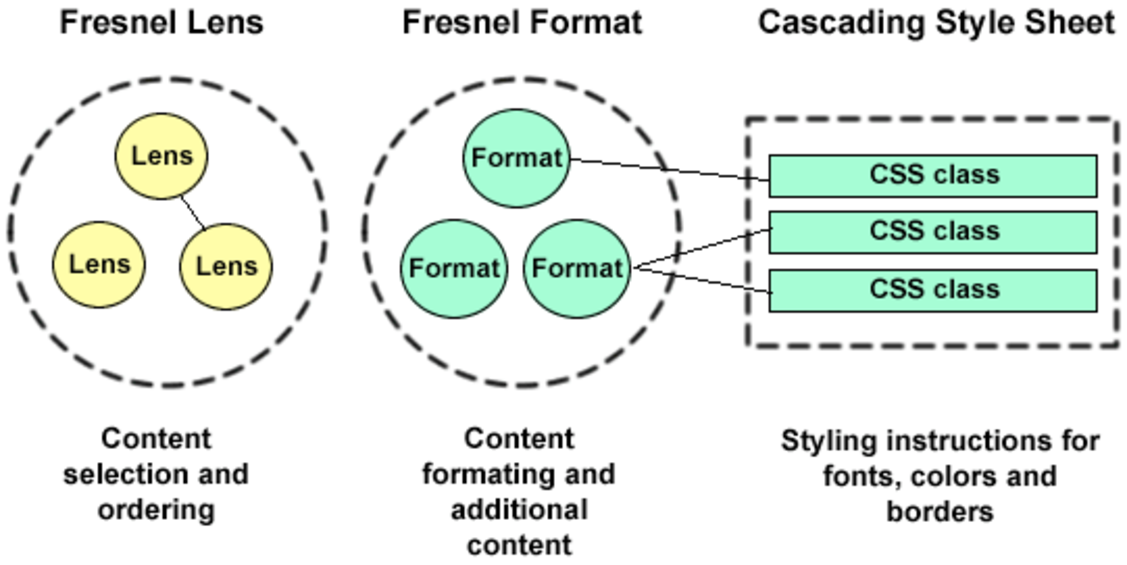
\includegraphics[width=8cm]{overview.pdf}
\caption{Fresnel foundational concepts}
\label{foundationalConceptsFig}
\end{center}
\end{figure}


%--------------------------------------------------------------------
\section{Fresnel Core Vocabulary Overview}
\label{fresnelov}

Fresnel is an RDF vocabulary, described by an OWL ontology \cite{fresnel05}. Fresnel presentation knowledge is thus expressed declaratively in RDF and relies on two foundational concepts: {\em lenses} and {\em formats} (see Figure \ref{foundationalConceptsFig}). Lenses specify which properties of RDF resources are shown and how these properties are ordered while formats indicate how to format content selected by lenses and optionally generate additional static content and hooks in the form of CSS class names that can be used to style the output through external CSS style sheets.

Figure \ref{exampleFig} shows a simple lens and associated formats used to present information about a person described with the FOAF vocabulary \cite{foaf}. This figure also shows a hypothetical rendering of such a resource, as an Horus \cite{horus} or Longwell-like browser could produce. Examples use the Notation 3 syntax \cite{N3}.

\begin{figure}
\begin{center}
\begin{tabular}{lp{4.5cm}}
\begin{small}
\begin{tt}
\begin{tabular}{ll}
(1) & :PersonLens a fresnel:Lens ;\\
(2) & ~~~~fresnel:classLensDomain foaf:Person ;\\
(3) & ~~~~fresnel:showProperties (\\
(4) & ~~~~~~~~foaf:name\\
(5) & ~~~~~~~~foaf:mbox\\
(6) & ~~~~~~~~foaf:depiction\\
(7) & ~~~~).\\
(8) & :nameFormat a fresnel:Format ; \\
(9) & ~~~~~~~fresnel:label "Name" ;\\
(10) & ~~~~~~~fresnel:propertyFormatDomain foaf:name .\\
(11) & :mboxFormat a fresnel:Format ;\\
(12) & ~~~~~~~fresnel:propertyFormatDomain foaf:mbox ;\\
(13) & ~~~~~~~fresnel:label "Mailbox" ;\\
(14) & ~~~~~~~fresnel:value fresnel:externalLink ;\\
(15) & ~~~~~~~fresnel:valueFormat [ fresnel:contentAfter "," ] .\\
(16) & :depictFormat a fresnel:Format ;\\
(17) & ~~~~~~~fresnel:propertyFormatDomain foaf:depiction ;\\
(18) & ~~~~~~~fresnel:label fresnel:none ;\\
(19) & ~~~~~~~fresnel:value fresnel:image .\\
\end{tabular}
\end{tt}
\end{small}
&
\begin{picture}(45,0.1)(0,0)\put(-27,65){\makebox(0,0){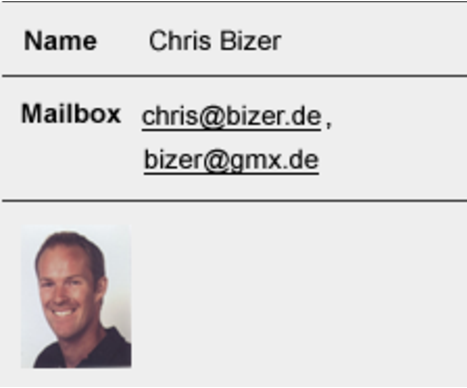
\includegraphics[width=4.2cm]{boxmodelexampleoutput.pdf}}}\end{picture} \\
\end{tabular}
\caption{A lens and some formats for presenting instances of class \rdf{foaf:Person}}
\label{exampleFig}
\end{center}
\end{figure}

\vspace{-1.5cm}

\subsection{Content selection}

The domain of a lens indicates the set of resources to which a lens applies (line 2). Property \rdf{showProperties} is used to specify what properties of these resources to show and in what order (lines 3-7). In this example, the values of both \rdf{classLensDomain} and \rdf{showProperties} are basic selectors, which take the form of plain URIs (represented here as qualified names), respectively identifying the class of resources and property types to select. More complex selection expressions can be written using either FSL or SPARQL (see section \ref{selectors}), making it possible to associate lenses with untyped RDF resources, which do occur in real-world models since \rdf{rdf:type} properties are not mandatory. Format domains can also be specified with one of these three solutions.

Fresnel Core provides additional constructs for specifying what properties of resources to display. The special value \rdf{fresnel:allProperties} can be used to avoid having to explicitly name each property that should be displayed. This value is also useful when the list of properties that can potentially be associated with resources handled by a lens is unknown to the lens' author but should nevertheless be displayed. When it appears as a member of the list of properties to be shown by a lens, \rdf{fresnel:allProperties} designates the set of properties that are not explicitly designated by other property URI references in the list, except for properties that appear in the list of properties to hide (\rdf{fresnel:hideProperties}). The extended lens vocabulary defines two other constructs to handle the potential irregularity of RDF data stemming from the fact that different authors might use similar terms coming from different vocabularies to make equivalent statements. Sets of such similar properties can be said to be \rdf{fresnel:alternateProperties}. For instance, \rdf{foaf:name}, \rdf{dc:title}, and \rdf{rdfs:label} could be considered by a lens as giving the same information about resources. A browser using this lens would then try to display the resources' \rdf{foaf:name}. If the latter did not exist, the browser would look for \rdf{dc:title} or \rdf{rdfs:label}. The second construct, \rdf{fresnel:mergeProperties}, is used to merge the values of related properties (e.g. \rdf{foaf:homepage} and \rdf{foaf:workHomepage}) into one single set of values that can later be formatted as a whole.

The presentation of property values is not limited to a single level, and recursive calls to lenses can be made to display details about the value of a property. Inserting the following lines in Figure \ref{exampleFig} between lines 6 and 7:\\
\begin{small}
\begin{tt}
\begin{tabular}{ll}
(6a) & ~~~[rdf:type fresnel:PropertyDetails ;\\
(6b) & ~~~~fresnel:property "foaf:knows[foaf:Person]"$^{\wedge\wedge}$fresnel:fslSelector;\\
(6c) & ~~~~fresnel:sublens :PersonLabelLens]\\
\end{tabular}
\end{tt}
\end{small}
\\tells the browser to render values of the property \rdf{foaf:knows}, which must be instances of \rdf{foaf:Person}, using another lens (\rdf{PersonLabelLens}). Infinite loops cau\-sed by recursive calls to the same lens are prevented by a closure mechanism.

\subsection{Content formatting}

The representation of selected information items mainly depends on the browser's representation paradigm (e.g. nested box layout, node-link diagrams, etc.) which defines the rendering method. The final rendering can be further customized by associating formatting instructions with elements of the representation.

Formats apply to resources, or to properties and their values, depending on the specified domain. The three example formats of Figure \ref{exampleFig} apply respectively to the properties \rdf{foaf:name}, \rdf{foaf:mbox} and \rdf{foaf:depiction} (lines 10,12,17). Formats can be used to set properties' labels (lines 9, 13, 18) and to indicate how to render values. For instance, line 14 indicates that \rdf{foaf:mbox} values should be rendered as clickable links (email addresses). Values of \rdf{foaf:depiction} should be fetched from the Web and rendered as bitmaps (line 19). Fresnel also defines default display methods in case such indications are not given by a format.

Property values can be grouped, and additional content such as commas (line 15) and an ending period can be specified to present multi-valued properties. CSS class names can also be associated with the various elements being formatted. These names appear in the output document and can be used to style the output by authoring and referencing CSS style sheets that use rules with the same class names as selectors.


%--------------------------------------------------------------------
\section{Fresnel Selectors}
\label{selectors}

Selection in Fresnel occurs when specifying the domain of a lens or format and when specifying what properties of a resource a lens should show. Such selection expressions identify elements of the RDF model to be presented; in other words, specific nodes and arcs in the graph. As we expect selection conditions to be of varying complexity, we allow them to be expressed using different languages in an attempt to balance expressive power against ease of use.

\subsection{Basic Selectors}

The simplest selectors, called basic selectors, take the form of plain URI references as shown in section \ref{fresnelov}. Depending on whether they are used as values of \rdf{fresnel:instan\-ceLensDomain} or \rdf{fresnel:classLensDomain}, these URI references are interpreted respectively either as:
\begin{itemize}
\item URI equality constraints (the resource to be selected should be identified by this URI),
\item or type constraints (the resources to be selected should be instances of the class identified by this URI).
\end{itemize}

Basic selectors are also used to identify properties, which are used for instance as values of \rdf{fresnel:showProperties} or \rdf{fresnel:alternateProperties}.

%In the following example, property \rdf{fresnel:lensDomain} indicates that this lens should be used to display instances of class \rdf{foaf:Person}, i.e., resources that have an rdf:type property pointing at class (or at a subclass of \footnote{Subclass and subproperty relationships must be taken into account by the selection mechanism, provided that an RDF Schema or OWL ontology is available at runtime 
%for the associated vocabulary.}) \rdf{foaf:Person}. Property \rdf{fresnel:showProperties} takes as its value a list of URIs referencing RDF property types. Properties \rdf{foaf:name} and \rdf{foaf:depiction} of resources displayed by this lens should be shown. 

%\begin{small}
%\begin{verbatim}
%:PersonLens a fresnel:Lens ; 
%    fresnel:lensDomain foaf:Person ; 
%    fresnel:showProperties (
%        foaf:name 
%        foaf:depiction
%    ).
%\end{verbatim}
%\end{small}

Basic selectors are easy to use but have very limited expressive power. For instance, they cannot be used to specify that a lens should apply to all instances of class \rdf{foaf:Person} that are the subject of at least five \rdf{foaf:knows} statements. More powerful languages are required to express such selection constraints.

\subsection{Languages for Complex Selection Expressions}

Fresnel presentation designers can use two different languages for expressing complex selection expressions. The first option is the SPARQL query language for RDF \cite{sparql05}. In the context of Fresnel, SPARQL queries must always return exactly one result set, meaning that only one variable is allowed in the query's SELECT clause. Figure \ref{fslsparqlExample}-a gives an example of a lens whose domain is defined by a SPARQL expression. Alternatively, designers who prefer a more XPath-like approach, which proved to be a well-adapted selector language for XSLT, can use the Fresnel Selector Language (FSL). FSL is a language for modeling traversal paths in RDF graphs, designed to address the specific requirements of a selector language for Fresnel. It does not pretend to be a full so-called RDFPath language (contrary to XPR \cite{xpr06}, an extension of FSL) but tries to be as simple as possible, both from usability and implementation perspectives. FSL is strongly inspired by XPath \cite{xpath}, reusing many of its concepts and syntactic constructs while adapting them to RDF's graph-based data model. RDF models are considered directed labeled graphs according to RDF Concepts and Abstract Syntax \cite{rdfcas04}. FSL is therefore fully independent from any serialization. A lens definition using two FSL expressions is shown in Figure \ref{fslsparqlExample}-b. More information about FSL, including its grammar, data model and semantics is available in the FSL specification \cite{fsl05}.

\begin{figure}
%\begin{center}
\begin{scriptsize}
\begin{verbatim}
# (a) Lens for John Doe's mailboxes    (SPARQL)
:PersonLens a fresnel:Lens ;
            fresnel:instanceLensDomain
              "SELECT ?mbox WHERE ( ?x foaf:name 'John Doe' )
                                  ( ?x foaf:mbox ?mbox )"^^fresnel:sparqlSelector .

# (b) Lens for foaf:Person instances that know at least five other resources  (FSL)
:PersonLens a fresnel:Lens ;
            fresnel:instanceLensDomain
                       "foaf:Person[count(foaf:knows) >= 5]"^^fresnel:fslSelector ;
# and which shows the foaf:name property of all foaf:Person
# instances known by the current resource.
            fresnel:showProperties (
                         "foaf:knows/foaf:Person/foaf:name"^^fresnel:fslSelector) .
\end{verbatim}
\end{scriptsize}
%\end{center}
\vspace{-1em}
\caption{Examples of SPARQL and FSL expressions used in Fresnel lens definitions}
\label{fslsparqlExample}
\vspace{-1em}
\end{figure}


Applications implementing Fresnel are required to support basic selectors, and we expect a reasonable share of them to support the two other languages: SPARQL is gaining momentum as a W3C recommendation, and four open-source Java implementations of FSL are already available\footnote{http://dev.w3.org/cvsweb/java/classes/org/w3c/IsaViz/fresnel/} for HP's Jena Semantic Web Toolkit\footnote{http://jena.sourceforge.net}, for IsaViz (providing a visual FSL debugger) and for different versions of the Sesame RDF database\footnote{http://openrdf.org}.


%--------------------------------------------------------------------
%--------------------------------------------------------------------
\section{Conclusion}

We have given an overview of Fresnel, a browser-independent, extensible vocabulary for modeling Semantic Web content presentation knowledge. Fresnel has been designed as a modularized, declarative language manipulating selection, formatting, and styling concepts that are applicable across representation paradigms, layout methods, and output formats. Fresnel core modules can be used to model presentation knowledge that is compatible and reusable between browsers and other types of Semantic Web information visualization~tools.

%I've added a ~ between the last two words to prevent tools from going on the next line.

Although core modules have been frozen for the time being, the Fresnel vocabulary remains a work in progress as new extension modules meeting special needs are being developed (e.g., for describing the {\em purpose} of lenses or adding new formatting capabilities). Extension modules are not necessarily aimed at being application- and paradigm-independent, as they might not be relevant in all cases; but their inclusion in Fresnel provides users with a unified framework for modeling presentation knowledge. 

Core modules are currently being implemented in various types of applications: SIMILE's Longwell \cite{simile} faceted browser, IsaViz \cite{isaviz} which represents RDF graphs as node-link diagrams, and Horus \cite{horus}, a PHP-based RDF browser. More information about Fresnel can be found on its web site\footnote{http://www.w3.org/2005/04/fresnel-info/}. Its development is an open, community-based effort and new contributors are welcome to participate in it.



%%%%%%%%%%%%%%%%%%%%%%%%%%%%%%%%%%%%%%%%%%%
% I'm temporarily using the \newpage and \vspace instructions to make sure
% that ACK and Refs fit on one page
%%%%%%%%%%%%%%%%%%%%%%%%%%%%%%%%%%%%%%%%%%%

\section*{Acknowledgments}

\vspace{-1mm}

\begin{small}
We would like to thank members of the SIMILE and Haystack projects at MIT for their valuable input, especially Stefano Mazzocchi, David Karger, Stephen Garland, David Huynh, Karun Bakshi, and the others who contributed to the discussion about Fresnel: Hannes Gassert, Jacco van Ossenbruggen, Dennis Quan, and Lloyd Rutledge.
\end{small}

\vspace{-3mm}

%
% ---- Bibliography ----
%

\bibliographystyle{splncs}
\bibliography{fresnel}

\end{document}
